\chapter{Methods}
\label{chp:methods}


%% Vi kan sikkert skrive litt om dette i metode

% \subsection{Version Control}
% \label{subsec:version-control}

% The use of \gls{git} as a version control system enables collaborative development by allowing multiple developers to work on the same codebase simultaneously. \gls{git} facilitates the maintenance of the code and provides a comprehensive history of all modifications made to the project. These changes are tracked within project containers known as \glspl{repository}, ensuring transparency and accountability throughout the development process. \cite{alphaefficiency:git}

% \subsubsection*{Branches}

% Git utilizes branches, which are independent lines of development within a repository. Branches allow developers to work on new features, fixes, or experiments without affecting the main codebase. Once changes in a branch are tested and finalized, they can be merged back into the main branch, ensuring a streamlined and controlled integration process. Branching supports parallel development and helps prevent conflicts by isolating work until it's ready for review and integration. \cite{git:branches}

\begin{center}
    \textit{Here, the development process and methodologies are described in detail. This includes the design and implementation of the desktop application, the selection of tools and frameworks, and the approach to solving the problem.}
\end{center}



\section{Machine Learning Models}
\label{sec:ml-models}

After conducting research into existing chess digitization methods, a publicly available solution developed by Peter Batchelor, Tom Richardson, and other contributors was discovered. This solution served as the foundation for the approach. It utilized two \glspl{cnn}: one for detecting chess pieces and another for locating the squares of the chessboard \cite{lichess:chesscam}. \\

Although the documentation for the models was limited, the necessary logic and structure of the models were already present in the repository itself. When additional clarifications were needed, they were obtained through direct communication with the original developers, ensuring that the intended use and functionality of the models were correctly understood. \\

The ChessCam repository provided multiple model formats, including PyTorch and ONNX. Before the models could be used, it was necessary to understand their expected inputs and outputs. Netron was employed to inspect the ONNX files and determine these details. \\

\newpage


\subsection{Piece Detection Model}
The piece detection model was responsible for identifying and classifying chess pieces on the board. It expected \textbf{input} in the format \textbf{[1, 3, 288, 480]}. \textbf{1} represented the batch size, i.e. the number of images processed at once, which was typically set to 1 during inference. \textbf{3} corresponded to the number of color channels (RGB), indicating that the image had to be in color. \textbf{288} and \textbf{480} denoted the height and width of the image in pixels, respectively. \\

The piece model output data in the format \textbf{[1, 16, 2835]}. \textbf{1} represented the batch size. \textbf{2835} represented the number of anchor boxes used in the detection. \textbf{16} consisted of two parts: \\

The first 4 values were offset values that adjusted the position and size of each anchor box to better align with a detected piece. These offsets were relative to the predefined anchor boxes, as illustrated in Table \ref{tab:piece-offset-table}.

\begin{table}[h]
    \centering
    \caption{Offset coordinates for each anchor box with regard to identifying chess pieces.}  % Caption moved to top
    \renewcommand{\arraystretch}{1.5} % Increase row height to allow text to be on top
    \begin{tabular}{lcccc}
        \toprule
        \textbf{Anchor box} & \textbf{xcenter} & \textbf{ycenter} & \textbf{width} & \textbf{height} \\
        \midrule
        Anchor box 1 & -3.23 & 0.57 & -0.12 & -0.34 \\
        Anchor box 2 & 0.51 & -0.63 & 4.15 & 1.27 \\
        Anchor box 3 & 7.71 & 0.29 & -0.11 & 2.45 \\
        ... & ... & ... & ... & ... \\
        Anchor box 2835 & -0.04 & 2.11 & 1.15 & 5.32 \\
        \bottomrule
    \end{tabular}
    \label{tab:piece-offset-table}
\end{table}


The remaining 12 values represented the probabilities for each possible piece type after the offset value had been applied. With 12 different piece types, the model output 12 probabilities for each anchor box. The classification labels are shown in Table \ref{tab:piece-label-table}. Table \ref{tab:piece-probability-table} presents the predicted probabilities for each label across all anchor boxes. \\

\begin{table}[ht]
\centering
\caption{Classification labels for the 12 chess piece types predicted by the model.}
\begin{tabular}{|c|c|}
\hline
\multicolumn{2}{|c|}{\textbf{Model Labels}} \\  % Adds a row at the top
\hline
\textbf{Black Pawn} & \textbf{White Pawn} \\
\textbf{Black Knight} & \textbf{White Knight} \\
\textbf{Black Bishop} & \textbf{White Bishop} \\
\textbf{Black Rook} & \textbf{White Rook} \\
\textbf{Black Queen} & \textbf{White Queen} \\
\textbf{Black King} & \textbf{White King} \\
\hline
\end{tabular}
\label{tab:piece-label-table}
\end{table} 

\\


\begin{table}[h]
    \centering
    \caption{Predicted class probabilities for each anchor box after applying the offsets.}  % Caption moved to top
    \renewcommand{\arraystretch}{1.5} % Increase row height to allow text to be on top
    \begin{tabular}{lcccc}
        \toprule
        \textbf{Anchor box} & \textbf{Black Pawn} & \textbf{White Pawn} & \textbf{Black Knight} & \textbf{...} \\
        \midrule
        Anchor box 1 & \raggedright 0.03 & \raggedright 0.71 & \raggedright 0.01 & ... \\
        Anchor box 2 & \raggedright 0.82 & \raggedright 0.02 & \raggedright 0.01 & ... \\
        Anchor box 3 & \raggedright 0.02 & \raggedright 0.01 & \raggedright 0.78 & ... \\
        ... & ... & ... & ... & ... \\
        Anchor box 2835 & \raggedright 0.01 & \raggedright 0.03 & \raggedright 0.05 & ... \\
        \bottomrule
    \end{tabular}
    \label{tab:piece-probability-table}
\end{table}

\newpage

To summarize, there were 2835 predefined anchor boxes spread across the image, each serving as a candidate location for detecting a chess piece. During training, the model learned to adjust these anchor boxes to better match the actual pieces on the board. It achieved this by predicting 4 offset values that modified the location and size of each anchor box. At runtime, for each anchor box, the model used these learned offsets and output 12 class probabilities, indicating the likelihood of each chess piece type being present at that location.

\newpage

\subsection{Corner Detection Model}
The corner detection model identified the points where the edges of the inner squares on the chessboard met, commonly referred to as intersection points. Up to 49 intersection points could be detected in a single image. These points are illustrated in Figure \ref{fig:xcorners-chessboard}.

\begin{figure}[h!]
    \centering
    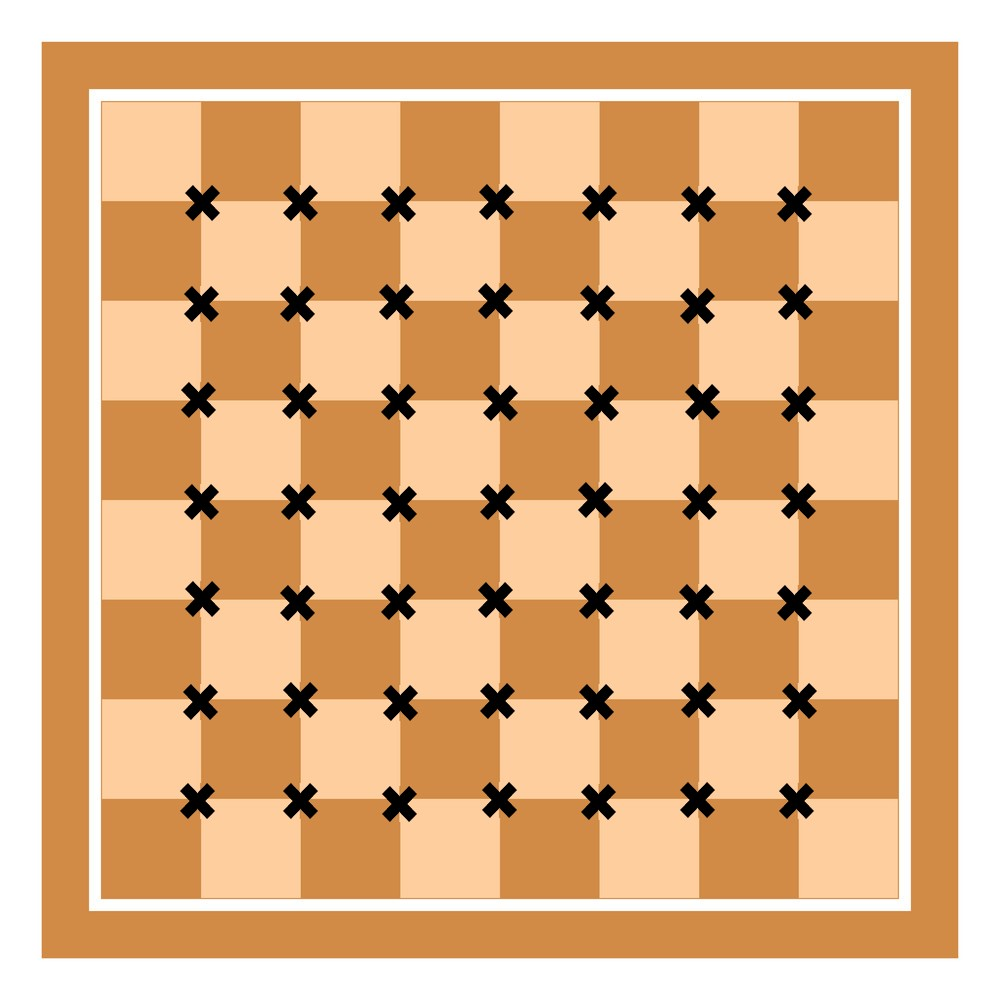
\includegraphics[width=0.75\linewidth]{figures/methods/ml-models/xcorners_chessboard.jpg}
    \caption[s]{Visualization of intersection points where the edges of the inner squares on the chessboard meet. The model identified and predicted these points. Up to 49 intersection points could be detected in a single image. \cite{vectorstock:chessboard-svg}}
    \label{fig:xcorners-chessboard}
\end{figure}

The input for the corner model was the same as the piece model: \textbf{[1, 3, 288, 480]}. The corner model output predictions in the format \textbf{[1, 5, 2835]}. \textbf{1} represented the batch size. \textbf{2835} represented the number of anchor boxes used in the detection. \textbf{5} consisted of two parts: \\

The first 4 values were offset values that adjusted the position and size of each anchor box, aligning it more accurately with a potential intersection point. These offsets were relative to the original anchor box coordinates, as shown in Table \ref{tab:corner-offset-table}.

\newpage

\begin{table}[h]
    \centering
    \caption{Offset coordinates for each anchor box with regard to identifying intersection points.}  % Caption moved to top
    \renewcommand{\arraystretch}{1.5} % Increase row height to allow text to be on top
    \begin{tabular}{lcccc}
        \toprule
        \textbf{Anchor box} & \textbf{xcenter} & \textbf{ycenter} & \textbf{width} & \textbf{height} \\
        \midrule
        Anchor box 1 & -1.43 & 3.27 & -0.52 & -2.21 \\
        Anchor box 2 & 2.51 & -7.61 & 0.15 & 4.17 \\
        Anchor box 3 & -3.71 & 1.49 & -4.21 & 2.45 \\
        ... & ... & ... & ... & ... \\
        Anchor box 2835 & -2.04 & 3.29 & -0.35 & 1.24 \\
        \bottomrule
    \end{tabular}
    \label{tab:corner-offset-table}
\end{table}

The final value was the probability that the adjusted anchor box corresponded to an intersection point on the chessboard, as illustrated in Table~\ref{tab:corner-probability-table}. \\

\begin{table}[h]
    \centering
    \caption{Predicted intersection probabilities for each anchor box after applying the offsets.}
    \renewcommand{\arraystretch}{1.5}
    \begin{tabular}{lc}
        \toprule
        \textbf{Anchor Box} & \textbf{Intersection Probability} \\
        \midrule
        Anchor Box 1 & 0.06 \\
        Anchor Box 2 & 0.91 \\
        Anchor Box 3 & 0.03 \\
        ... & ... \\
        Anchor Box 2835 & 0.87 \\
        \bottomrule
    \end{tabular}
    \label{tab:corner-probability-table}
\end{table}


\newpage


\subsection{Combining the models}

To track chess piece movements, the first step was to identify the individual squares of the chessboard. Once the squares were identified, each detected piece needed to be mapped to its corresponding square. This required determining the outer corners of the chessboard. With the corners identified, the board was divided into an 8x8 grid of equally sized squares. Since the distance between the corners was known and all squares in the grid are of uniform size, the centers of the squares could be precisely calculated. For each square, only the center point would be used for subsequent mapping, as shown in Figure~\ref{fig:chessboard-centers}.



\begin{figure}[h!]
    \centering
    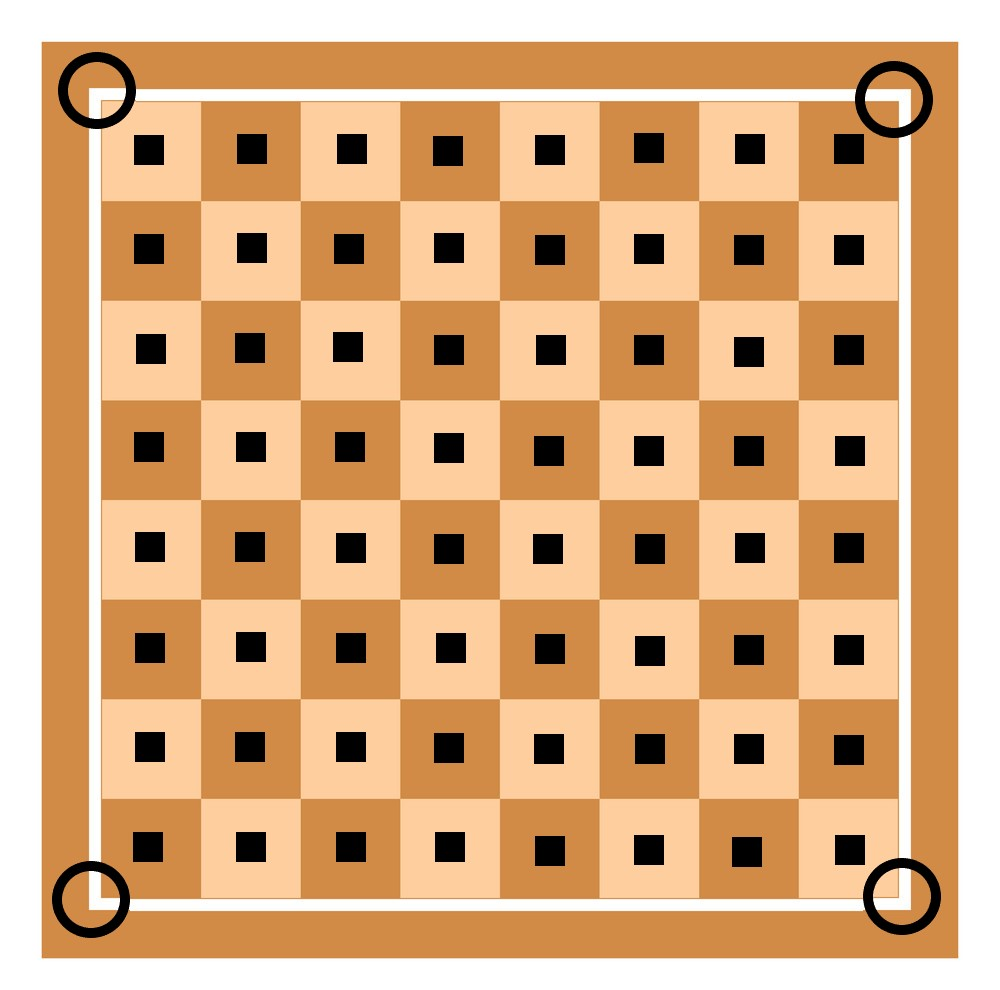
\includegraphics[width=0.75\linewidth]{figures/methods/ml-models/outer_corners_centers_chessboard.jpg}
    \caption[S]{Visualization of the outer corners of the chessboard and the centers of each individual square, forming an 8x8 grid. \cite{vectorstock:chessboard-svg}}
    \label{fig:chessboard-centers}
\end{figure}


The bottom center of each piece’s bounding box was selected as its representative location, as highlighted in Figure~\ref{fig:bbox-black-pawn}. Each detected piece was then mapped to the nearest square center based on the minimum euclidean distance.  This approach made it possible to accurately assign each piece to a specific square on the chessboard.



\newpage

\begin{figure}[h!]
    \centering
    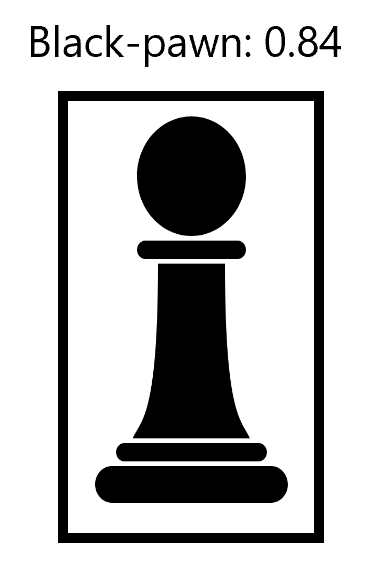
\includegraphics[width=0.25\linewidth]{figures/methods/ml-models/black-pawn.png}
    \caption[FIX]{Example of a detected chess piece with its classification confidence. The bottom center of the bounding box was used as the reference point for mapping the piece to its corresponding square. \cite{svgrepo:black-pawn-svg}}
    \label{fig:bbox-black-pawn}
\end{figure}

\subsubsection*{Implementation}

The essence of how it works:
So how was this done? The camera first captures a video frame, which is then processed by both models. Each frame is resized to the required input dimensions, normalized so that pixel values fall between 0 and 1, and converted to the correct format and data type expected by the models, in this case resized to the expected input format {1,3,288,480} and returns the 
[1, 16, 2835] for the piece model
[1, 5, 2835] for the corner model.

We now have 2835 locations for both the intersection points and piece locations. We wish to extract the best predictions from these dense outputs. To do this, we first filter out low-confidence predictions based on a score threshold. Then, we apply \gls{nms} to eliminate overlapping detections, ensuring that only the most confident and distinct predictions are kept.

To do this, we apply post-processing techniques, most importantly Non-Maximum Suppression (NMS), which helps eliminate overlapping or low-confidence predictions. This step ensures that only the most likely and distinct piece locations and board intersections (x-corners) are retained.

Inside this function, the first step is to identify potential quadrilateral shapes that could represent the board's four corners. This is done by applying Delaunay triangulation on the detected x_corners to find a set of possible quads. A Delaunay triangulation ensures that the x_corners are used efficiently to form triangles, from which we can identify quadrilaterals. The get_quads function is used here to find such quads by iterating over the triangles and attempting to connect shared vertices to form four-sided polygons.

Once a list of potential quads is generated, each quad is scored which evaluates how well the quad fits with the original x_corners. The quad with the highest score is selected as the most likely representation of the board corners.

Next, we apply a perspective transformation to map the detected corners onto a regular grid. This is done by first calculating an inverse matrix of the transformation used to generate the corner locations, and then applying the inverse transformation to the predicted corners. The result is a set of warped corner coordinates that can be used to estimate the true position of the board on the screen.

Finally, the predicted corners are clamped to ensure that their values lie within the valid range for the image dimensions (width and height), ensuring no corner falls outside the image.

To summarize, the x_corners are processed by first identifying candidate quads through Delaunay triangulation, then evaluating each quad's suitability using scoring, and finally refining the corners using a perspective transformation. This series of steps helps accurately extract the four board corners from the intersection points, which can then be used for further processing.

Finally, labels are assigned to the corners of the chessboard. The centers of the black and white pieces are calculated, and the board is rotated in four possible ways (90-degree shifts). For each rotation, the midpoints of the white and black sides are calculated, and the distance between these midpoints and the calculated piece centers is measured. The rotation that results in the smallest distance, meaning the one that best aligns with the piece centers, is selected. The labels "a1", "h1", "a8", and "h8" are then assigned to the four corners based on the correct orientation, and the labeled corners are returned.




To identify candidate quadrilaterals on the chessboard, the implementation first performs Delaunay triangulation over the set of detected corner points. It then searches for pairs of adjacent triangles—triangles that share two vertices—and combines their points to form four-point quads. This method restricts the candidates to geometrically relevant regions made up of neighboring points, avoiding the need to evaluate all possible 4-point combinations, which would be computationally expensive and less accurate.


\begin{subfigure}[h!]{0.9\linewidth} \centering 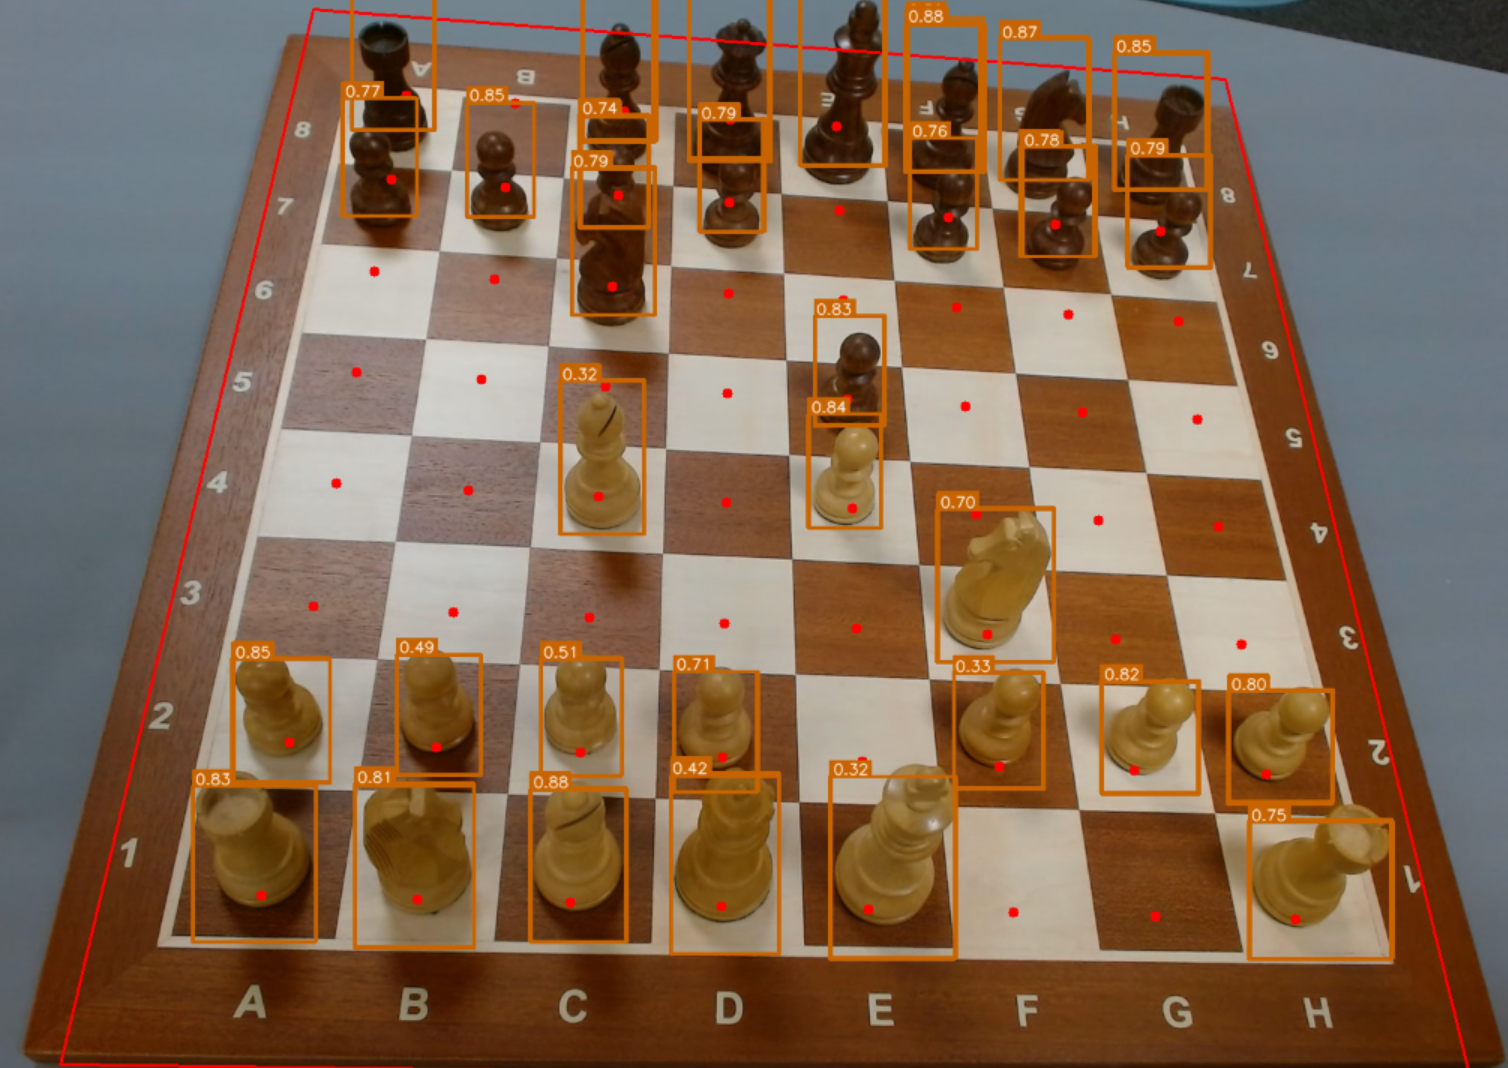
\includegraphics[width=\linewidth]{figures/methods/ml-models/piece-model.png} \caption{Tournament View} \end{subfigure}

\newpage


\section{Agile Methodology}
\label{sec:development-methodology}

The team organized their work into bi-weekly \textbf{sprints}, each culminating in a status report and retrospective. At the beginning of each sprint, the product backlog was reviewed to prioritize tasks for the upcoming sprint. Sprint goals were then set, and each team member outlined the tasks they planned to complete before the next meeting. The team reviewed completed tasks to assess progress. For any incomplete tasks, potential causes were discussed, and strategies for addressing them were devised. At the end of each sprint, retrospectives provided an opportunity for the team to reflect on their collaboration and identify areas for improvement. \\

To manage and track tasks, the team utilized GitHub’s \textbf{Issue Board}. Issues were categorized as follows: \textit{Enhancement} for new features or improvements, \textit{Documentation} for adding explanations or improving code safety, \textit{Bug} for errors or unexpected behaviors, and \textit{Task} for general tasks. Each issue was assigned to one or more team members to clarify responsibilities. The Issue Board was organized into four columns: \textit{No Status}, \textit{To Do}, \textit{In Progress}, and \textit{Done}, providing a clear visual overview of progress. \\

For \textbf{code review}, the team used GitHub pull requests. Each issue was worked on in a separate branch, enabling team members to review and discuss contributions before merging them into the main codebase.


% Jeg kommenterer disse ut ettersom jeg ikke helt vet hva som er ønsket skal stå under disse
%\subsubsection*{Product Owner}

%\subsubsection*{Supervisor}


\section{Architecture}
\label{subsec:diagrams}

To provide a comprehensive understanding of the system architecture and interaction flow, several \gls{uml} diagrams were created. These diagrams model different aspects of the live chess game digitization system, from component interactions and activity flow to user roles and use cases.

\subsubsection*{Sequence Diagram}
\label{subsubsec:sequence-diagram}

The sequence diagram, shown in Figure \ref{fig:sequence}, illustrates the chronological flow of interactions between the system components and external actors. It begins with the Admin initiating the game recording by setting up the camera, which captures and streams the board state to a local processing unit. This unit continuously detects and validates moves, updating the user interface accordingly. Users, from remote devices, can spectate the game in real time or save it as a \gls{pgn} file. The diagram emphasizes the communication between hardware (camera and local machine) and the \gls{ui}, highlighting how physical chess games are digitized and broadcasted.

\newpage

\begin{figure}[h!]
    \centering
    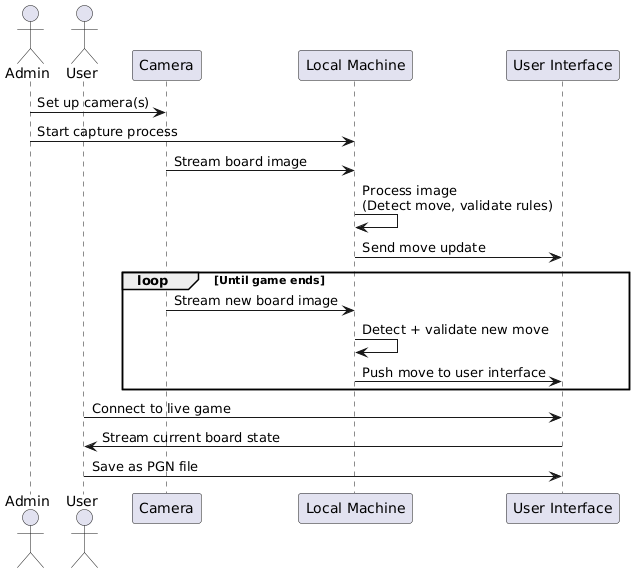
\includegraphics[width=0.75\linewidth]{figures/methods/uml/sequence.png}
    \caption[Sequence Diagram]{Sequence Diagram}
    \label{fig:sequence}
\end{figure}

\subsubsection*{Use-Case Diagram}
\label{subsubsec:use-case-diagram}

The use-case diagram, shown in Figure \ref{fig:use-case}, identifies the system’s main actors and the primary functionalities they interact with. Admins are responsible for hardware setup and initiating the game recording process. The system autonomously handles move detection, validation, and \gls{ui} updates. Users, on the other hand, access the game remotely to spectate or download \gls{pgn} files. This diagram provides a clear overview of who interacts with the system and what capabilities are exposed, forming the basis for understanding system requirements and user expectations.

\begin{figure}[h!]
    \centering
    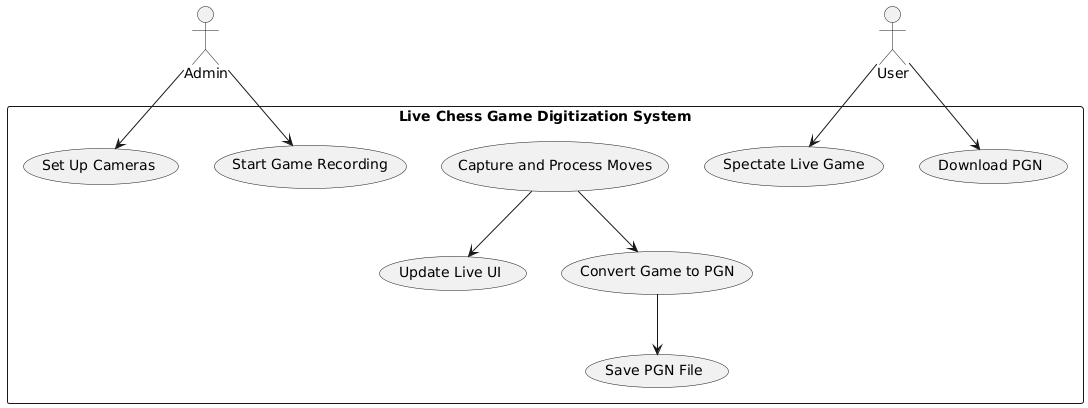
\includegraphics[width=0.75\linewidth]{figures/methods/uml/use-case.png}
    \caption{Use-Case Diagram}
    \label{fig:use-case}
\end{figure}

\begin{figure}[h!]
    \subsubsection*{Activity Diagram}
    \label{subsubsec:activity-diagram}
    
    \centering
    \begin{minipage}[t]{0.5\textwidth}
        \vspace{0pt}
        The activity diagram, shown in Figure \ref{fig:activity}, provides a high-level overview of the operational workflow during a chess game session. It models the continuous loop of capturing board states, detecting and validating moves, and updating the game state until the game ends. If a move is invalid, the system flags it but does not terminate the session. Once the game concludes, it is converted into a standard \gls{pgn} format. This diagram emphasizes the logical flow and decision-making process, reflecting the system’s role in automating and maintaining the integrity of live digitization.
    \end{minipage}
    \hfill
    \begin{minipage}[t]{0.45\textwidth}
        \vspace{0pt}
        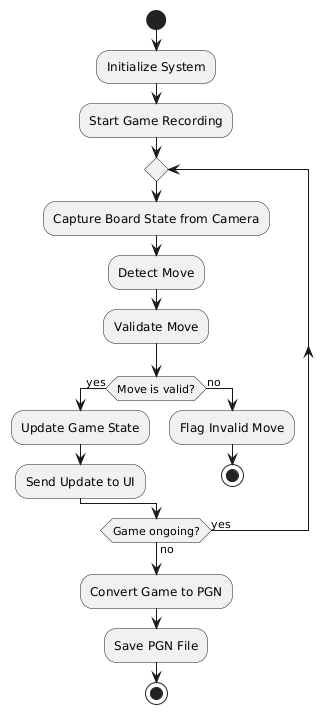
\includegraphics[width=\linewidth]{figures/methods/uml/activity-2.png}
        \caption[Activity Diagram]{Activity Diagram}
        \label{fig:activity}
    \end{minipage}
\end{figure}

\subsection{Wireframes}
\label{subsec:wireframe}

\subsubsection*{Control Panel}

The Control Panel is a desktop interface for tournament organizers to manage the digitization of multiple physical chess boards. It follows a simple three-step workflow:

\begin{enumerate}
\item \textbf{Select Number of Cameras:} Specify the number of boards to monitor, which determines how many camera feeds are initialized (Figure \ref{fig:control-panel-1}).
\item \textbf{Start Cameras and Digitization:} Launches the camera feeds, board state recognition, and move validation (Figure \ref{fig:control-panel-2}).
\item \textbf{Restart Boards for New Round:} Resets all boards at the end of a round, preparing the system for the next games (Figure \ref{fig:control-panel-3}).
\end{enumerate}

The interface is minimal and task-focused, enabling efficient system setup and management with little technical effort.

\begin{figure}[h!]
    \centering
    \begin{subfigure}[h!]{0.40\linewidth}
        \centering
        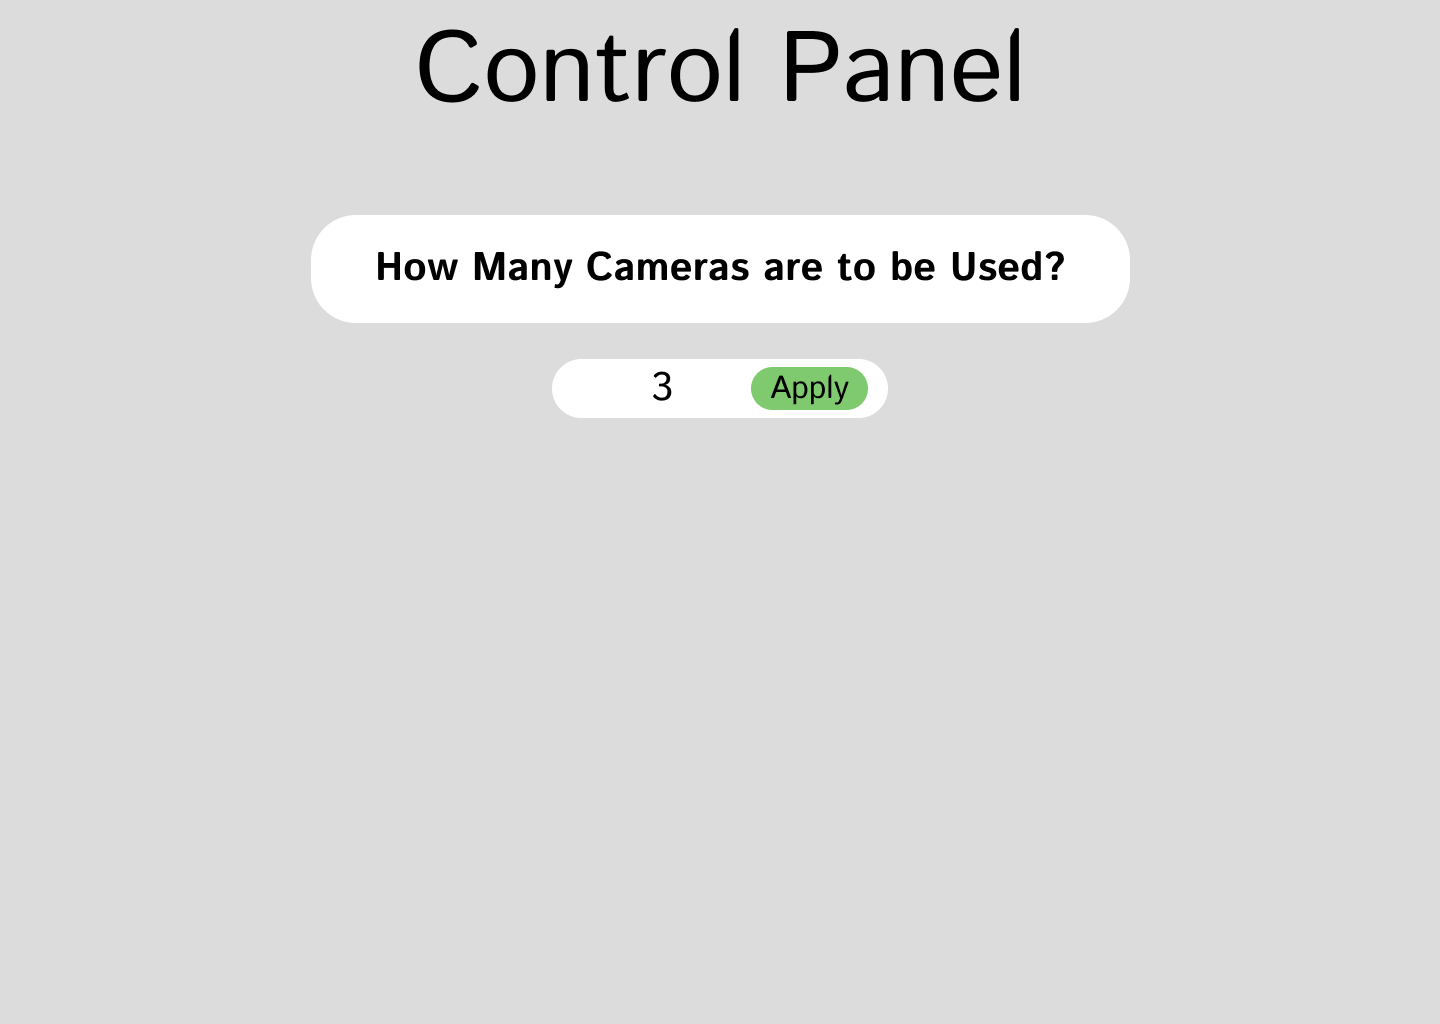
\includegraphics[width=\linewidth]{figures/methods/wireframes/control-panel-1.png}
        \caption{Step 1}
        \label{fig:control-panel-1}
    \end{subfigure}
    \hfill
    \begin{subfigure}[h!]{0.40\linewidth}
        \centering
        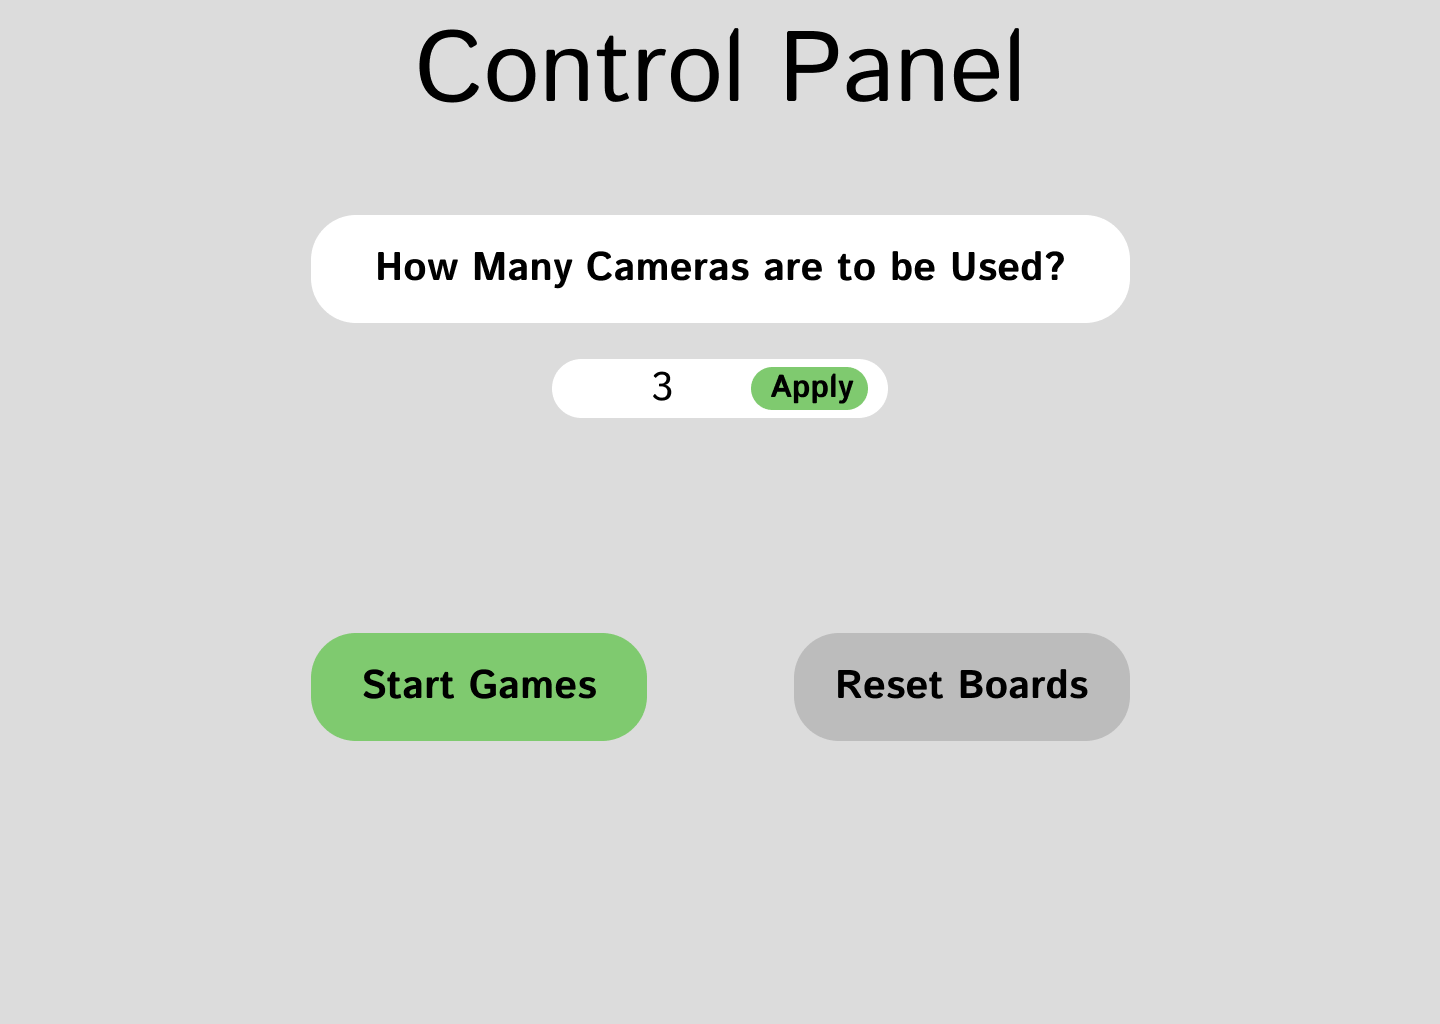
\includegraphics[width=\linewidth]{figures/methods/wireframes/control-panel-2.png}
        \caption{Step 2}
        \label{fig:control-panel-2}
    \end{subfigure}

    \begin{subfigure}[h!]{0.40\linewidth}
        \centering
        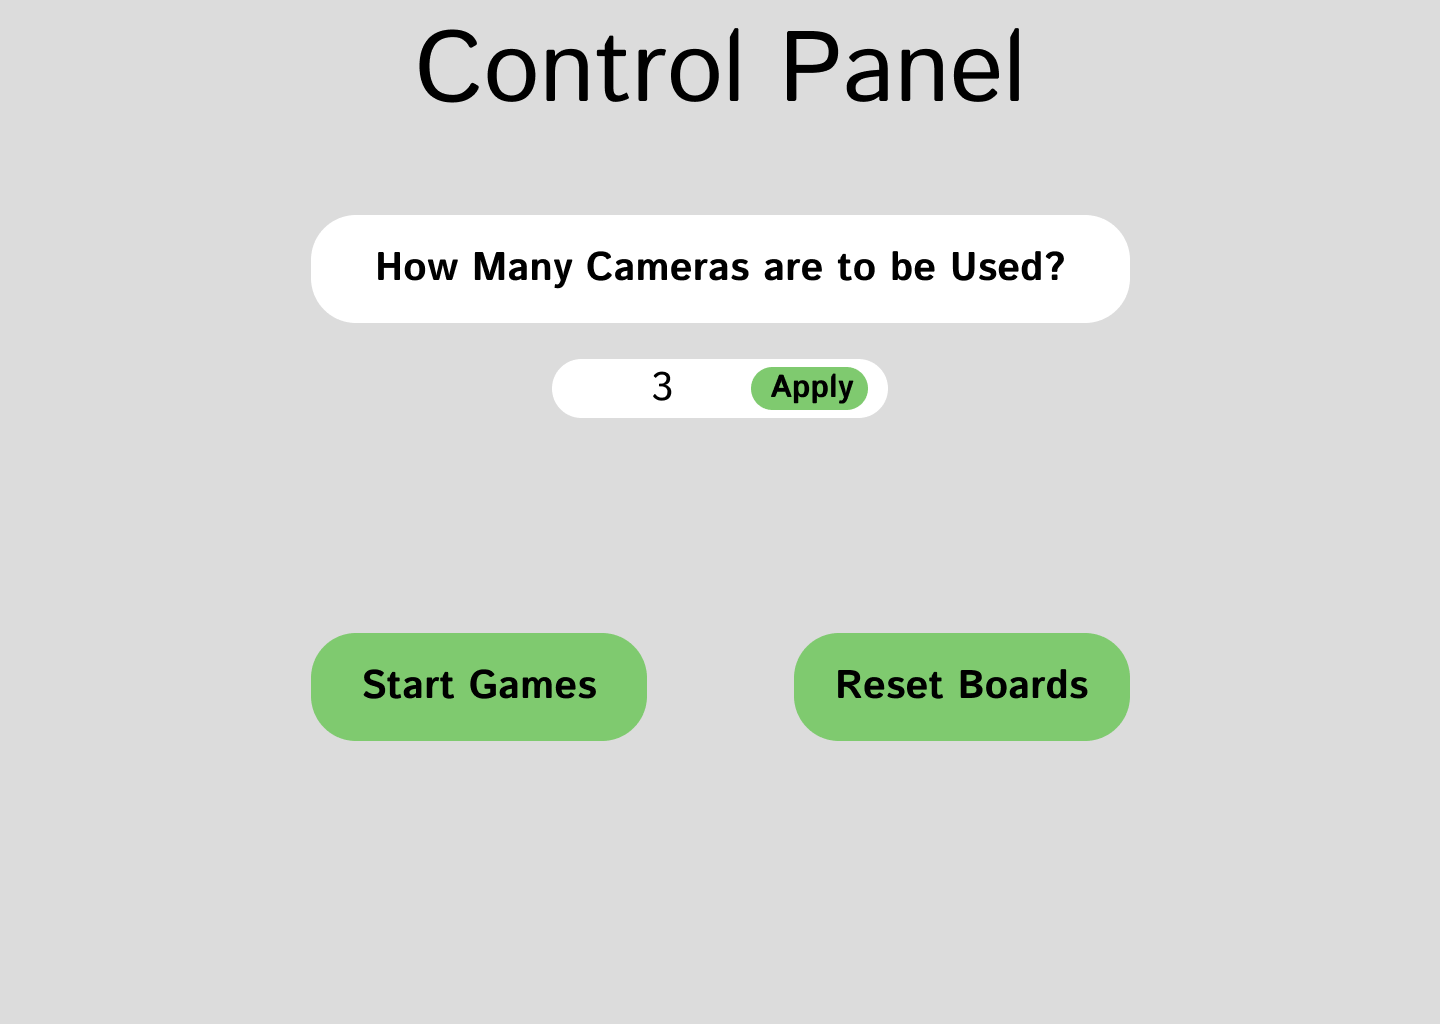
\includegraphics[width=\linewidth]{figures/methods/wireframes/control-panel-3.png}
        \caption{Step 3}
        \label{fig:control-panel-3}
    \end{subfigure}
    
    \caption{Control Panel wireframes showing sequential interaction steps}
    \label{fig:control-panel-group}
\end{figure}


\begin{figure}[h!]
\subsubsection*{Desktop View}
    \centering
    \begin{subfigure}[h!]{0.40\linewidth}
        \centering
        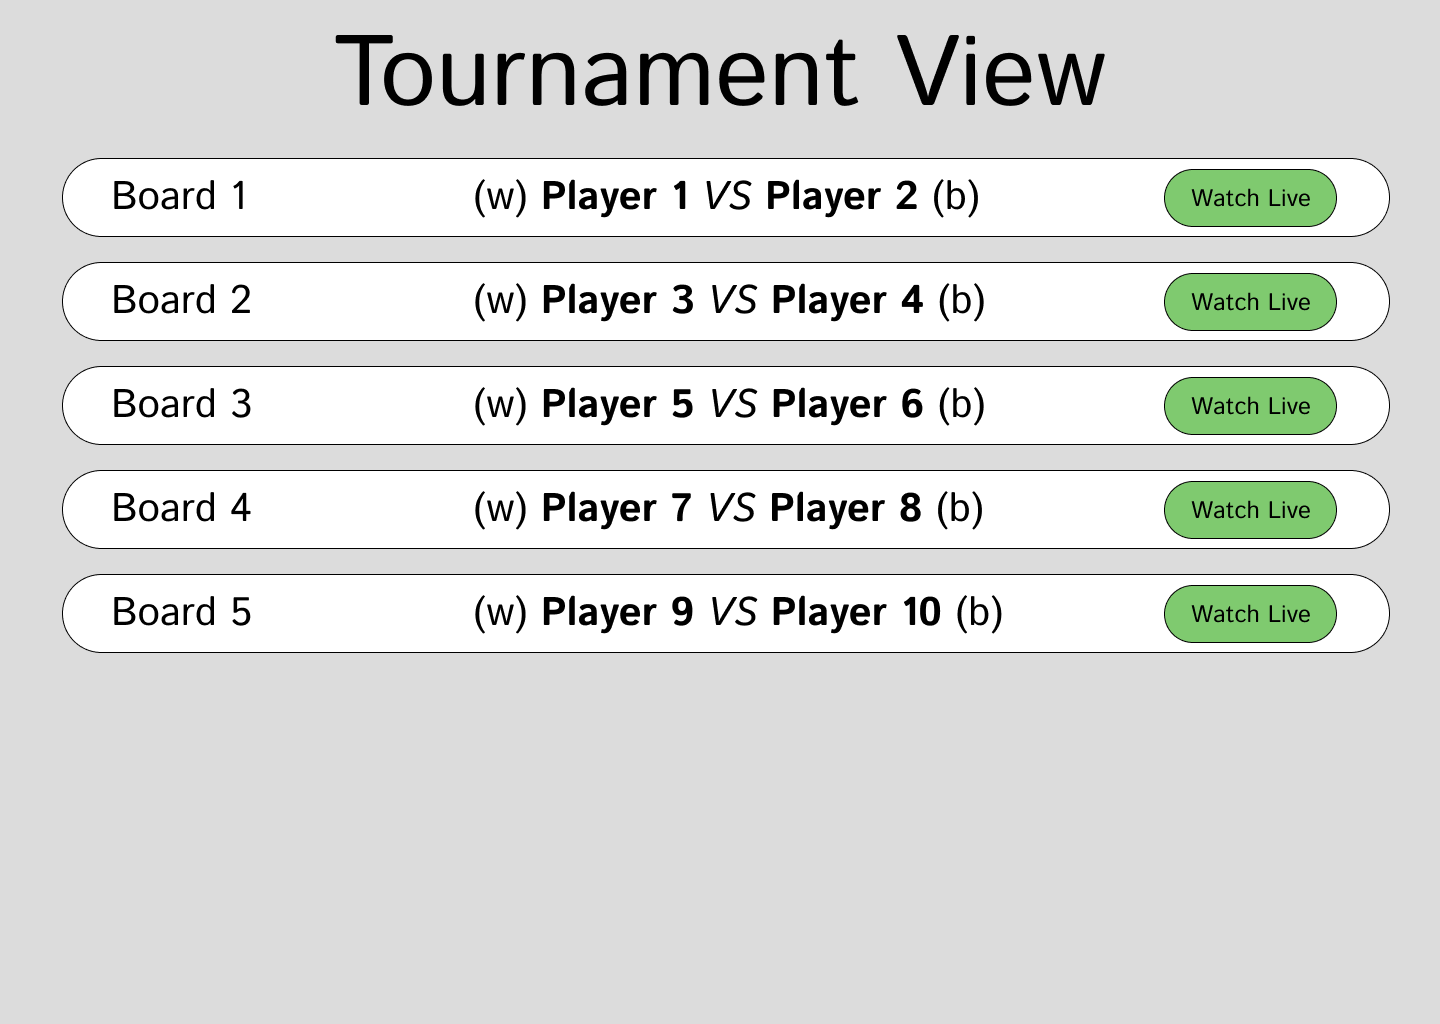
\includegraphics[width=\linewidth]{figures/methods/wireframes/desktop-tournament-view.png}
        \caption{Tournament View}
        \label{fig:desktoop-tournament-view}
    \end{subfigure}
    \hfill
    \begin{subfigure}[h!]{0.40\linewidth}
        \centering
        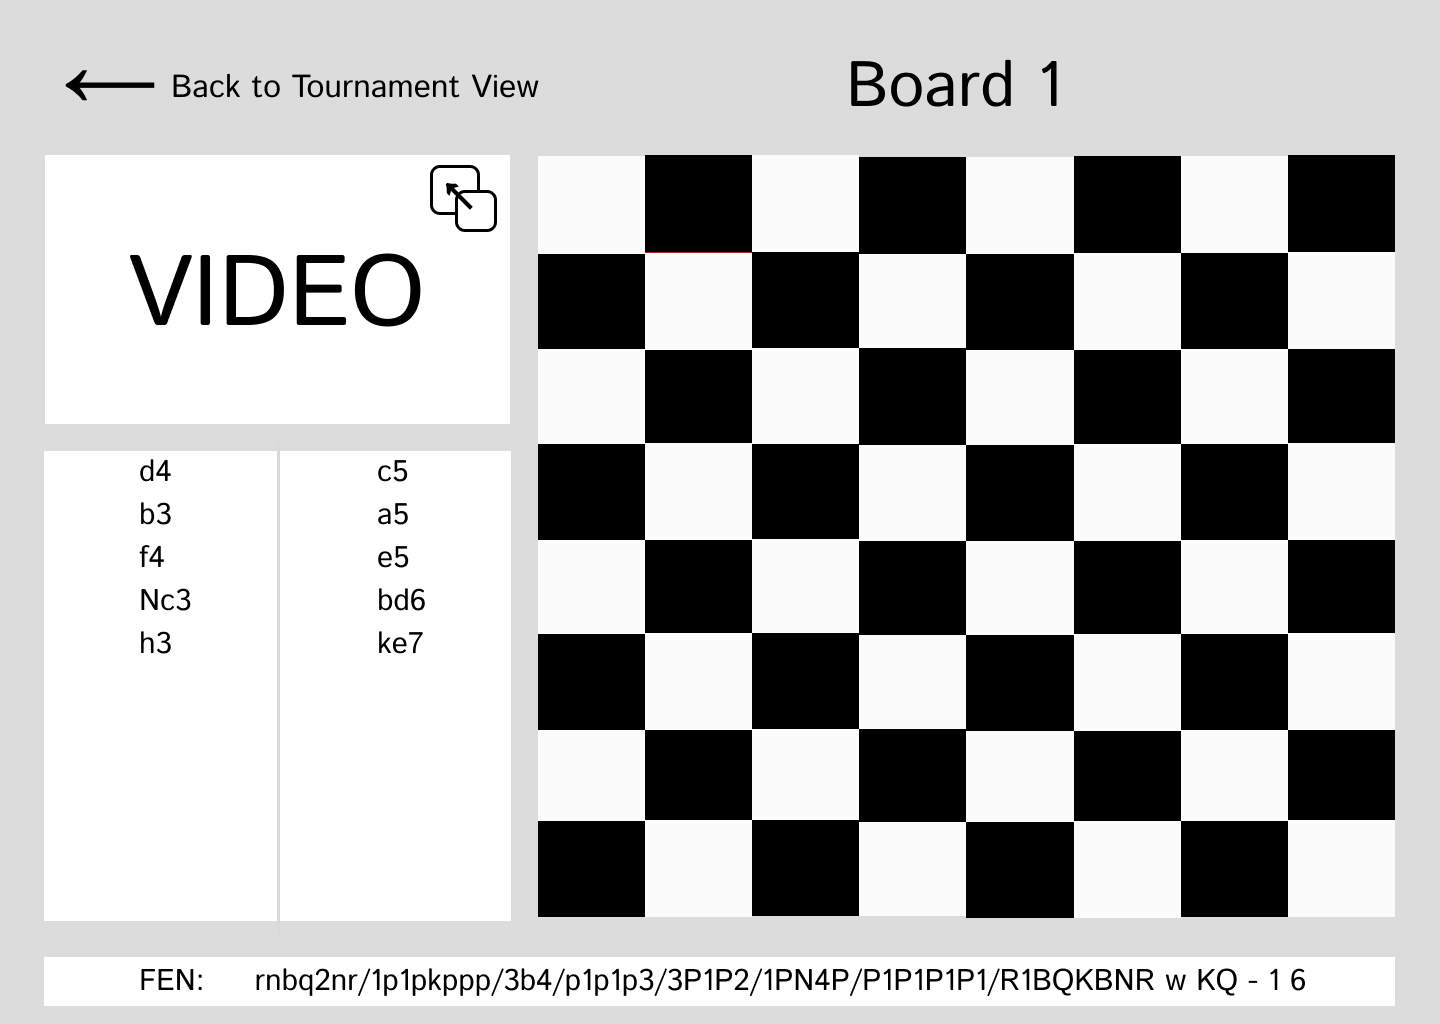
\includegraphics[width=\linewidth]{figures/methods/wireframes/desktop-board-view.png}
        \caption{Board View}
        \label{fig:desktop-board-view}
    \end{subfigure}

    \begin{subfigure}[h!]{0.40\linewidth}
        \centering
        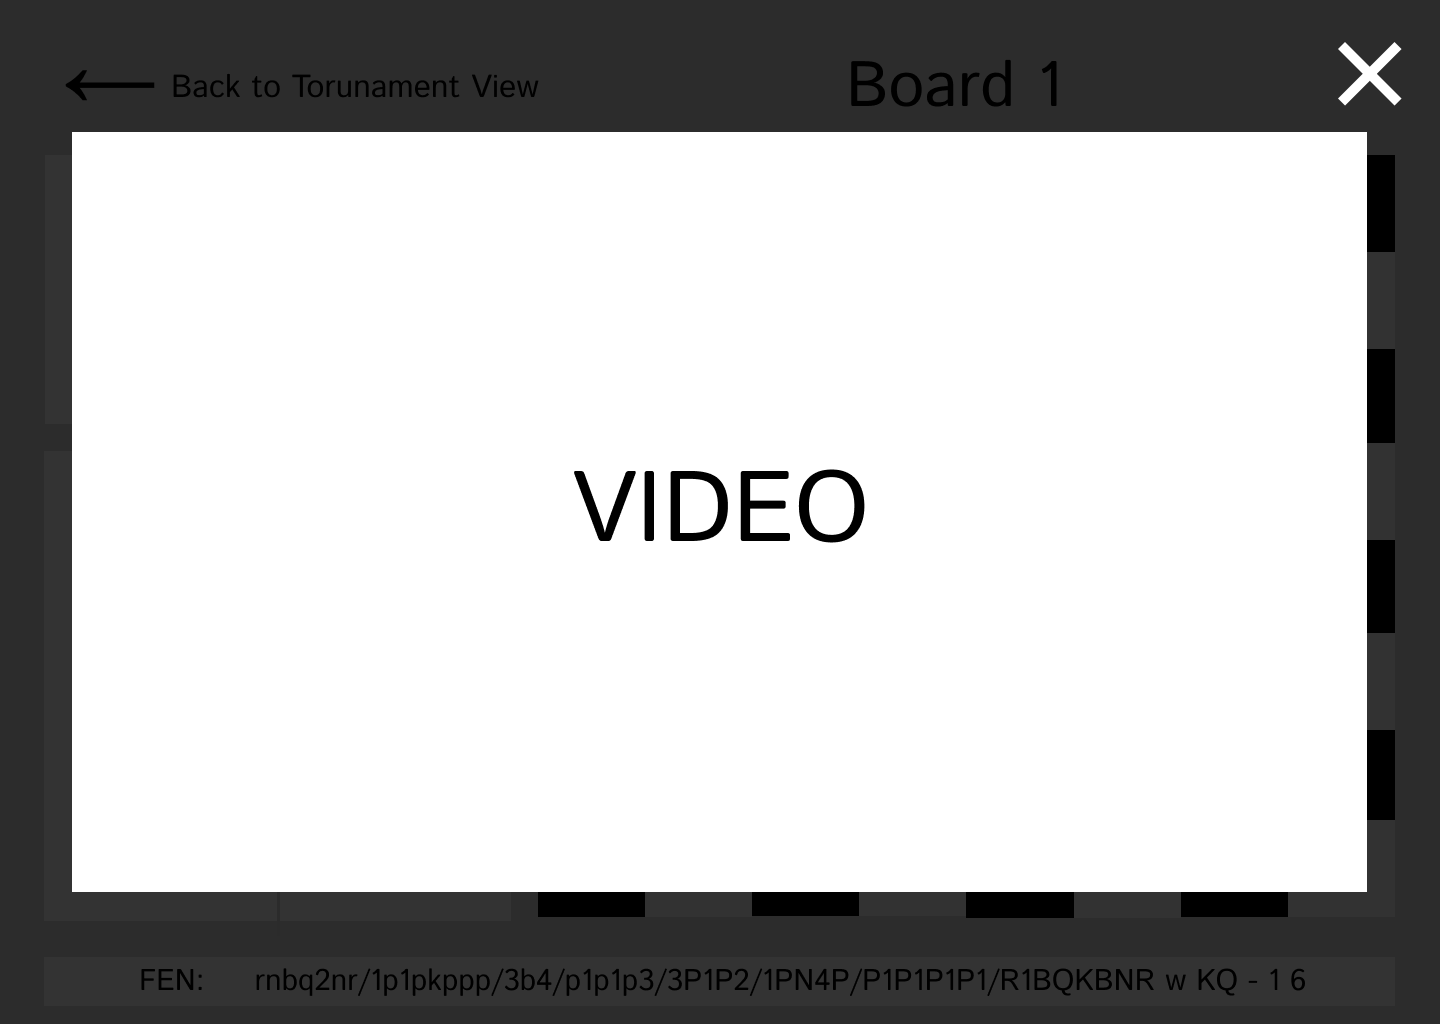
\includegraphics[width=\linewidth]{figures/methods/wireframes/desktop-full-screen-video-view.png}
        \caption{Fullscreen Video Feed}
        \label{fig:desktop-fullscreen-video}
    \end{subfigure}
    
    \caption{Desktop client-side view wireframes}
    \label{fig:desktop-view-group}
\end{figure}

\begin{figure}[h!]
\subsubsection*{Phone View}
    \centering
    \begin{subfigure}[h!]{0.2\linewidth}
        \centering
        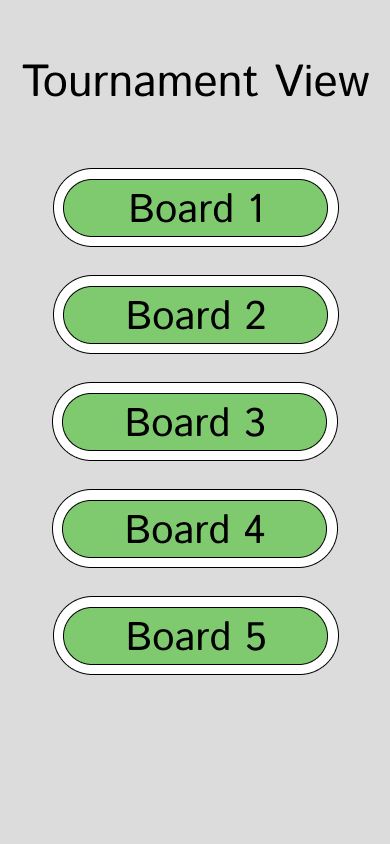
\includegraphics[width=\linewidth]{figures/methods/wireframes/phone-tournament-view.png}
        \caption{Tournament View}
        \label{fig:phone-tournament-view}
    \end{subfigure}
    \hfill
    \begin{subfigure}[h!]{0.2\linewidth}
        \centering
        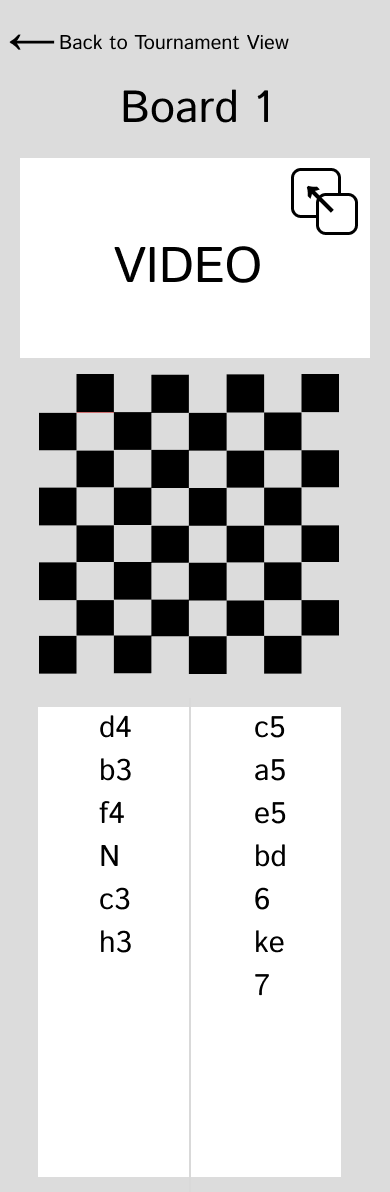
\includegraphics[width=\linewidth]{figures/methods/wireframes/phone-board-view.png}
        \caption{Board View}
        \label{fig:phone-board-view}
    \end{subfigure}
    \hfill
    \begin{subfigure}[h!]{0.2\linewidth}
        \centering
        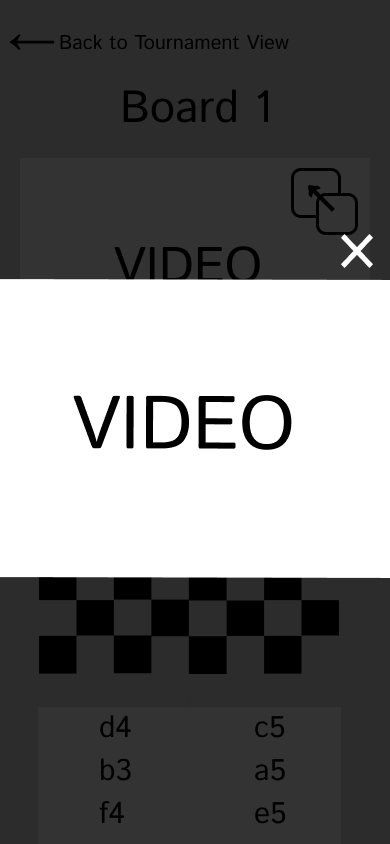
\includegraphics[width=\linewidth]{figures/methods/wireframes/phone-full-screen-video-view-vertical.png}
        \caption{Vertical Fullscreen Video Feed}
        \label{fig:phone-fullscreen-video-vertical}
    \end{subfigure}
    \hfill
    \begin{subfigure}[h!]{0.2\linewidth}
        \centering
        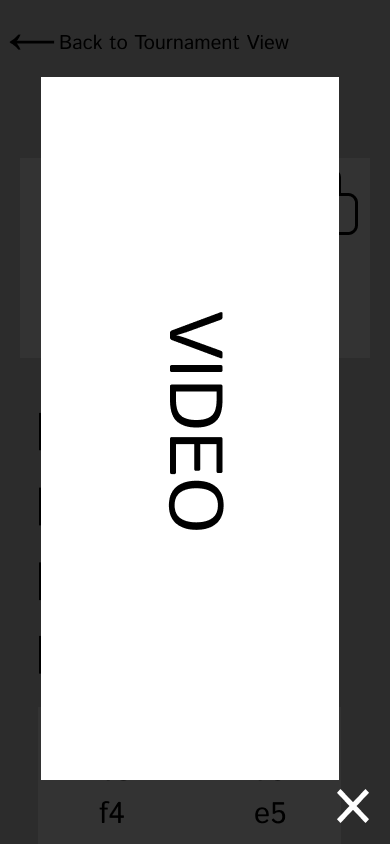
\includegraphics[width=\linewidth]{figures/methods/wireframes/phone-full-screen-video-view-horizontal.png}
        \caption{Horizontal Fullscreen Video Feed}
        \label{fig:phone-fullscreen-video-horizontal}
    \end{subfigure}
    
    \caption{Phone client-side view wireframes}
    \label{fig:phone-view-group}
\end{figure}

\section{Tools and Platforms}
\label{sec:tools-and-platforms}

\subsection*{Development Tools}
\label{subsec:development-tools}

\begin{itemize}
    \item \textbf{\gls{vscode}} was used as the primary development environment due to its support for multiple programming languages and extensions.
\item \textbf{Postman} was employed for testing and validating RESTful \glspl{api}, utilizing built-in JavaScript-based test snippets.
\item \textbf{Netron.app} was used to visualize neural network architectures during the evaluation phase.
\item \textbf{Git} facilitated version control and collaboration throughout the development process.
\item \textbf{\glspl{llm}} (e.g., ChatGPT) were consulted to review code and provide suggestions, functioning as a collaborative assistant.
\item \textbf{Lighthouse} was used to evaluate and improve the performance and accessibility of the developed web interface.
\end{itemize}.

\subsection*{Collaboration Tools}
\label{subsec:collaboration-and-design-tools}

\begin{itemize}
    \item \textbf{GitHub} was used for its built-in project management tool, which allowed the team to create an Issue Board for easy issue tracking. It was also used for code reviews and version control management.
    
    \item \textbf{Figma} was used as a tool for sketching and creating wireframes.
    
    \item \textbf{OneDrive} was used as a platform for storing and sharing files.
    
    \item \textbf{Overleaf} was used as the platform for writing the report, utilizing its LaTeX support to efficiently compose and format the thesis.
\end{itemize}


\section{Technology Stack}
\label{sec:technology-stack}

\subsection*{Backend}
\subsubsection*{Python libraries}

\begin{itemize}
    \item \textbf{chess} – Used for move generation, validation, and parsing of chess game formats. \cite{python:chess}
    \item \textbf{FastAPI} – Web framework used to develop RESTful APIs for backend services. \cite{python:fastapi}
    \item \textbf{numpy} – Core package for numerical operations. \cite{python:numpy}
    \item \textbf{onnxruntime} Used for running pre-trained machine learning models. \cite{python:onnx}
    \item \textbf{opencv-python} Utilized for computer vision tasks. \cite{python:opencv}
    \item \textbf{requests} – Used to handle HTTP communication. \cite{python:requests}
    \item \textbf{scipy} – Employed for scientific and numerical computations. \cite{python:scipy}
    \item \textbf{tensorflow}, Used to build and execute machine learning models. \cite{python:tensorflow}
\end{itemize}


\subsection*{Frontend}
\subsubsection*{TypeScript libraries}

\begin{itemize}
    \item \textbf{Vite} is a fast frontend build tool of web applications. \cite{ts:vite}
    
    \item \textbf{React} builds user interfaces out of individual pieces called components. \cite{ts:react}
    
    \item \textbf{@vitejs/plugin-react-swc} Speeds up the Vite development server. \cite{ts:swc}
    
    \item \textbf{chess.ts} a Typescript chess library for chess move generation/validation, piece placement/movement, and check/checkmate/draw detection \cite{ts:chess}
    
    \item \textbf{react-dom} serves as the entry point to the DOM and server renderers for React. \cite{ts:react-dom}
\end{itemize}

\section{Testing}
\label{sec:testing}

\subsection{Model testing}
\label{subsec:model-testing}

The performance of the machine learning model was evaluated through 100 test games. Five distinct chess openings were selected, with 10 games played per opening on each of two board types: plastic and wooden. This resulted in 50 games per board type. Each game consisted of 15 full moves, corresponding to 15 moves by white and 15 moves by black. \\

Each move was logged as either successful or unsuccessful. A 30-second window was provided for the model to detect and transmit each move, starting from the moment the move was made \gls{otb}. If the model failed to detect the move within this time frame, or if it detected the wrong move, it was marked as unsuccessful. The game concluded either when a move was marked unsuccessful or all 15 full moves had been completed. \\

The webcam was mounted above the board at an angle of approximately 60–70\si{\degree}
 relative to the table surface. The white pieces were placed on the left side of the camera's field of view, and the black pieces on the right.

\begin{figure}[h!]
    \centering
    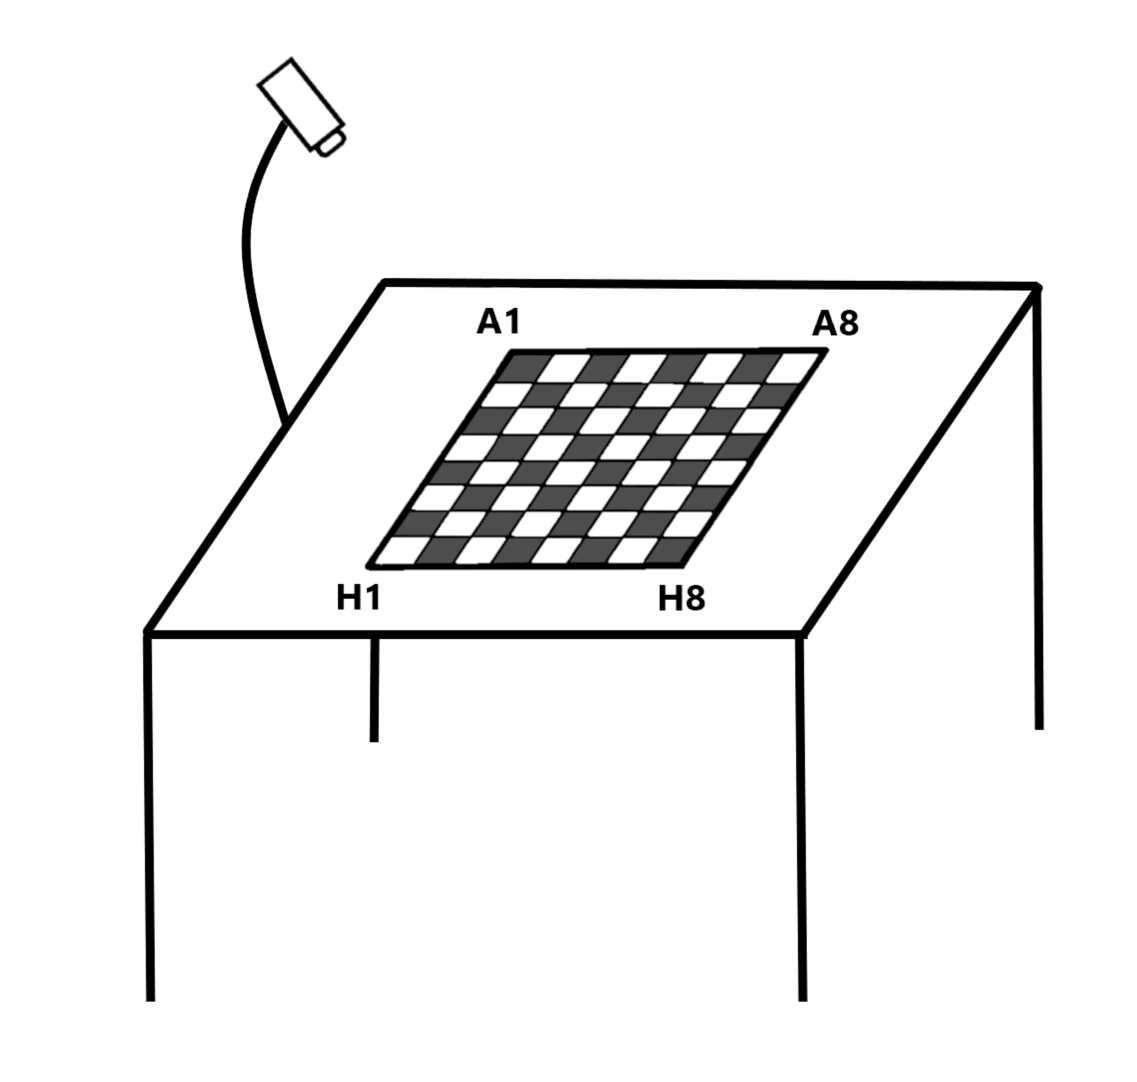
\includegraphics[width=0.75\linewidth]{figures/methods/testing/setup.png}
    \caption[Setup during testing]{Physical setup during testing, showing the board, webcam position, and piece orientation.}
    \label{fig:setup}
\end{figure}

\newpage



\subsection{Wireframe testing}
\label{subsubsec:user-centered-design}

The following processes align with the principles discussed in  Subsection~\ref{subsec:usability-testing} 
outlined in Chapter~\ref{chp:theory}. At the beginning of the design process, the group conducted wireframe testing with a diverse set of users. This included participants of varying age groups from young to elderly as well as both chess players and non-chess players. The goal was to evaluate whether users found the interface intuitive and whether the sizing and layout were appropriate. \\

All participants were given the same context before starting the test: 

\begin{quote}
\textit{You are viewing a chess game between two companions you know. You visit the tournament organizer's website and come across this webpage.}
\end{quote}

Participants were then either given specific tasks to perform within the application or asked to explore freely, mimicking a real-world scenario. This approach aimed to identify how naturally users could navigate and understand the application without explicit instruction. \\

After completing their interaction with the application, participants filled out an anonymous feedback form. The form included the following questions:

\begin{itemize}
    \item \textit{On a scale from 1 to 5, how satisfied are you with the overall experience of the application?}
    \item \textit{On a scale from 1 to 5, how satisfied are you with the Tournament View page?}
    \item \textit{On a scale from 1 to 5, how satisfied are you with the Board View page?}
    \item \textit{Do you have any feedback, suggestions for improvement, or features you would like to see added?}
\end{itemize}

See Subsection \ref{subsec:wireframe} for the final tested wireframe.

\newpage

\subsection{Color palette testing}
\label{subsubsec:color-palette}

In selecting the application's color palette, the group opted for a variation of blue. This choice was influenced by the symbolic associations of the color blue, which is often linked to imagination, intelligence, and wisdom \cite{blue} traits that are relevant to the game of chess \cite{chess:ppqty, chess:chess-and-creativity}. \\

To identify the most suitable stylistic direction, several versions of the application were developed, each showcasing a distinct color palette. These prototypes were printed and displayed in a shared space, allowing individuals from diverse backgrounds to view and compare them. \\

Participants were invited to vote for their preferred versions via a form. Each participant was allowed up to three votes and had the option to leave comments. For instance, some expressed a preference for the light mode from palette \#08 and the dark mode from palette \#07, while others favored the board design from palette \#05 or the move-highlighting style from palette \#14. \\

Rather than selecting a single predefined palette, the final color scheme was assembled by combining the most highly rated elements across the top-voted variations. This approach allowed for a more tailored and user-informed visual design (See Figure \ref{fig:color-palette-results} for the vote results). \\

\begin{figure}[h!]
    \centering
    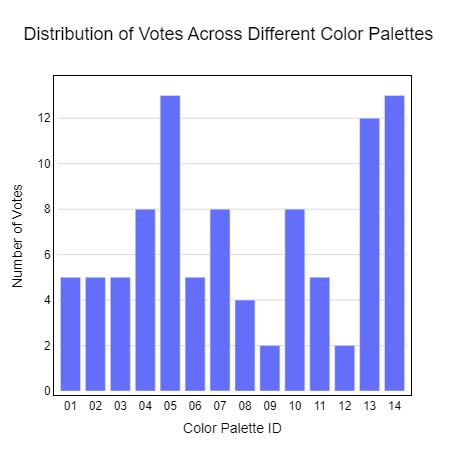
\includegraphics[width=0.75\linewidth]{figures/methods/color-palette-results.png}
    \caption{Distribution of Votes Across Different Color Palettes}
    \label{fig:color-palette-results}
\end{figure}

See Appendix~\ref{app:color-palettes} for the full set of tested color palettes.